\documentclass[12pt]{article}

\usepackage[margin=2cm]{geometry}
\usepackage{amsmath}
\usepackage{multicol}
\usepackage{nopageno}
\usepackage{SIunits}
\usepackage{graphicx}
\usepackage{enumerate}
\usepackage{enumitem}
%\usepackage{mathabx}
\usepackage{wasysym}


% for making bond drawings
\usepackage{chemfig}
% Global bond settings
\setchemfig{
  atom sep=18pt,               % fixed bond length
  double bond sep=2pt,       % spacing between the two bars
  bond style={line width=0.8pt}
}


% for centering figures on page while in an enumerated/itemized list:
\usepackage{changepage} % in the preamble
\makeatletter
\newenvironment{centerinpage}
  {%
    \par\noindent
    \hspace*{-\@totalleftmargin}% back to page margin (covers all nested list indents)
    \begin{minipage}{\textwidth}% fixed to page width (ignores widened \linewidth)
      \centering
  }
  {%
    \end{minipage}\par
  }
\makeatother

%%%%%%%%%%%%%%%%%%%%%%%%%%%%%%%%%%%%%%%%%%%%%%%%%%%%%
% For putting links in the document (both to sections and hyperlinks)
\usepackage{hyperref}
\usepackage{url}
\hypersetup{
    colorlinks=true,     % false: boxed links; true: colored links
    linkcolor=red,       % color of internal links
    citecolor=blue,      % color of links to bibliography
    filecolor=blue,      % color of file links
    urlcolor=blue        % color of external links
}
% below, use \url{http://www.nytimes.com} (they will be urlcolor)
%%%%%%%%%%%%%%%%%%%%%%%%%%%%%%%%%%%%%%%%%%%%%%%%%%%%%


%%%%%%%%%%%%%%%%%%%%%%%%%%%%%%%%%%%%%%%%%%%%%%%%%%%%%
% for the events page boxes

% boxed regions
\usepackage{tcolorbox}
\tcbuselibrary{skins,breakable}

% fonts & spacing
\usepackage{lmodern}
\usepackage{microtype}
\usepackage{calc}


% small helper macros (adjust these)
\newcommand{\boxheight}{4.2cm}   % height for each event box
\newcommand{\boxfont}{\scriptsize} % change to \tiny or \footnotesize as desired
\newcommand{\linelen}{0.95\linewidth} % timeline line length

%%%%%%%%%%%%%%%%%%%%%%%%%%%%%%%%%%%%%%%%%%%%%%%%%%%%%
\newcommand{\rmd}{\ensuremath{{\rm d}}}
%\newcommand{\vv}[1]{\ensuremath{\vec{#1}}}
\newcommand{\vv}[1]{\ensuremath{\mathbf{#1}}}
\newcommand{\ee}[1]{\ensuremath{\mathbf{e}_{#1}}}
%%%%%%%%%%%%%%%%%%%%%%%%%%%%%%%%%%%%%%%%%%%%%%%%%%%%%



\begin{document}

\begin{center}
{\Large Climate Forcing and Timescales}
\end{center}
%%%%%%%%%%%%%%%%%%%%%%%%%%%%%%%%%%%%%%%%%%%%%%%%
%%%%%%%%%%%%%      overview         %%%%%%%%%%%%%%%%%%%%%
%%%%%%%%%%%%%%%%%%%%%%%%%%%%%%%%%%%%%%%%%%%%%%%%


%
%\newpage
%%%%%%%%%%%%%%%%%%%%%%%%%%%%%%%%%%%%%%%%%%%%%%%%
%%%%%%%%%%%%%      questions         %%%%%%%%%%%%%%%%%%%%%
%%%%%%%%%%%%%%%%%%%%%%%%%%%%%%%%%%%%%%%%%%%%%%%%

\begin{enumerate}

\item  {\bf Forcing, non-equilibrium, and return to equilibrium}
	%
	\begin{enumerate}
	\item Using the information from this week's reading ({\em Dessler}, Chapter 6) and lecture, give a precise definition of {\bf radiative forcing} (RF).  Recall that it is a difference of two fluxes.  What are its units?
	\item Explain the {\em meaning} of radiative forcing in the context of climate (radiative) equilibrium.  Make reference to our prior work using energy flow/flux diagrams, and in particular the relationship of forcing to {\em equilibrium}. Explain the sequence of energy flux diagrams in Dessler's Figure 6.1 (reproduced here in Figure \ref{fig:dessler-fig6-1}).  What is the value (and units) of the radiative forcing imposed by the sudden atmosphere?
	\item Repeat the calculation example done by Dessler in Section 6.3.1. Assume that the solar flux initially has its standard value\footnote{Remember that this value is $F_\text{sun} = \frac{S}{4} (1 - \alpha)$, where $S=\unit{1360}{\joule/\second/\meter^2}$ is the Solar Constant, and $\alpha = 0.3$ is the albedo.}  of \unit{238}{\watt/\meter^2}.  Then, because of an orbital event, the Sun's flux increases by \unit{1}{\watt/\meter^2}, i.e., there is a radiative forcing of $\unit{+1}{\watt/\meter^2}$.  If the Earth's original equilibrium temperature (assuming no atmosphere) was \unit{254.55}{\kelvin}, what will be the new temperature after it returns to equilibrium?
	\item The radiative forcing induced by all of the human carbon dioxide production since 1750 (changing the atmospheric concentration from \unit{280}{ppm} to \unit{425}{ppm}) is about \unit{+2.2}{\watt/\meter^2}. The {\bf climate sensitivity} --- the forcing induced by a doubling of atmospheric carbon dioxide --- is about \unit{+4.0}{\watt/\meter^2}.  Using your answer to part (c), which gave an estimate of the temperature increase per \unit{1}{\watt/\meter^2} of forcing, what are the corresponding temperature increase\footnote{Feedbacks in the climate system (e.g., ice melt $\rightarrow$ decreasing albedo $\rightarrow$ increasing $F_\text{sun}$, see {\em Dessler} Section 6.3.2) amplify the climate sensitivity.  Current models incorporating all known effects estimate climate sensitivity to be about $\unit{3}{\kelvin} = 3\degree$C, with a likely range ($\sim70\%$ probability of being in) 2.6 to $4\degree$C.} predicted by these forcings for a no-atmosphere Earth?
	\end{enumerate}

\item {\bf Timescales of atmospheric carbon dioxide and temperature increase}
	%
	\begin{enumerate}
	\item The change in atmospheric carbon dioxide over the past 70 years (the ``Keeling Curve'') is shown in Figure \ref{fig:keeling-curve}.  Let's try to characterize that data by plotting it ourselves. 
		%
		\begin{itemize}
		\item First make a table with columns [t(yr), C(ppm), $\log_{10}$(C)]. Then choose about 5 points from the Keeling Curve data and record the values in your table, also calculating the logarithm of the concentration, C, value in your calculator.
		\item Take a regular sheet of graph paper and plot $\log_{10}(C)$ vs time. Be sure to choose your axis ranges so that you can fill most of the paper.
		\item Draw a best fit line to your plotted data and find its slope.
		\end{itemize}
		%
	When a quantity is increasing exponentially, it can be seen as a straight line on a log vs linear plot.  Does this data show evidence of exponential growth?  
	\item For an exponentially growing quantity, we can assign a constant ``doubling time''  to the growth rate.  This value is found as 
		%
		\begin{equation*}
		t_\text{double} = \frac{ \log_{10} (2) }{ \text{slope} }
		\end{equation*}
		%
	where ``slope'' is the slope of the log-linear plot.  Using this equation and your result from part (a), find the doubling time for atmospheric carbon dioxide.  
	\item Considering a longer-time plot of carbon dioxide in the atmosphere (Figure \ref{fig:co2-emissions-and-atmosphere}) and assuming that the exponential growth rate held over this whole period.  When do you expect we will double the value of carbon dioxide from 1750?
	\end{enumerate}
	
	
\newpage

\item ({\bf Not used in F2025}) Consider the graphs in Figure \ref{fig:jeevanjee-2025-review_fig1}. The top graph shows the effect of an annual 1\% increase in $\text{CO}_2$ up to doubling.  The bottom shows that the temperature is, model-predicted, to be proportional to the cumulative amount of emissions.
	

\end{enumerate}

\newpage

%%%%%%%%%%%%%%%%%%%%%%%%%%%%%%
%\mbox{}
%\newpage
%%%%%%%%%%%%%%%%%%%%%%%%%%%%%%

%%%%%%%%%%%%%%%%%%%%%%%%%%%%%%%%%%%%%%%%%%%%%%%%%%%%
%%%%%%%%%%               milankovitch wikimedai            %%%%%%%%%%%%%
%%%%%%%%%%%%%%%%%%%%%%%%%%%%%%%%%%%%%%%%%%%%%%%%%%%%

%%%%%%%%%%%%%%%%%%%%%%%%%%%%%%%%
\newpage

\begin{figure}
\centering
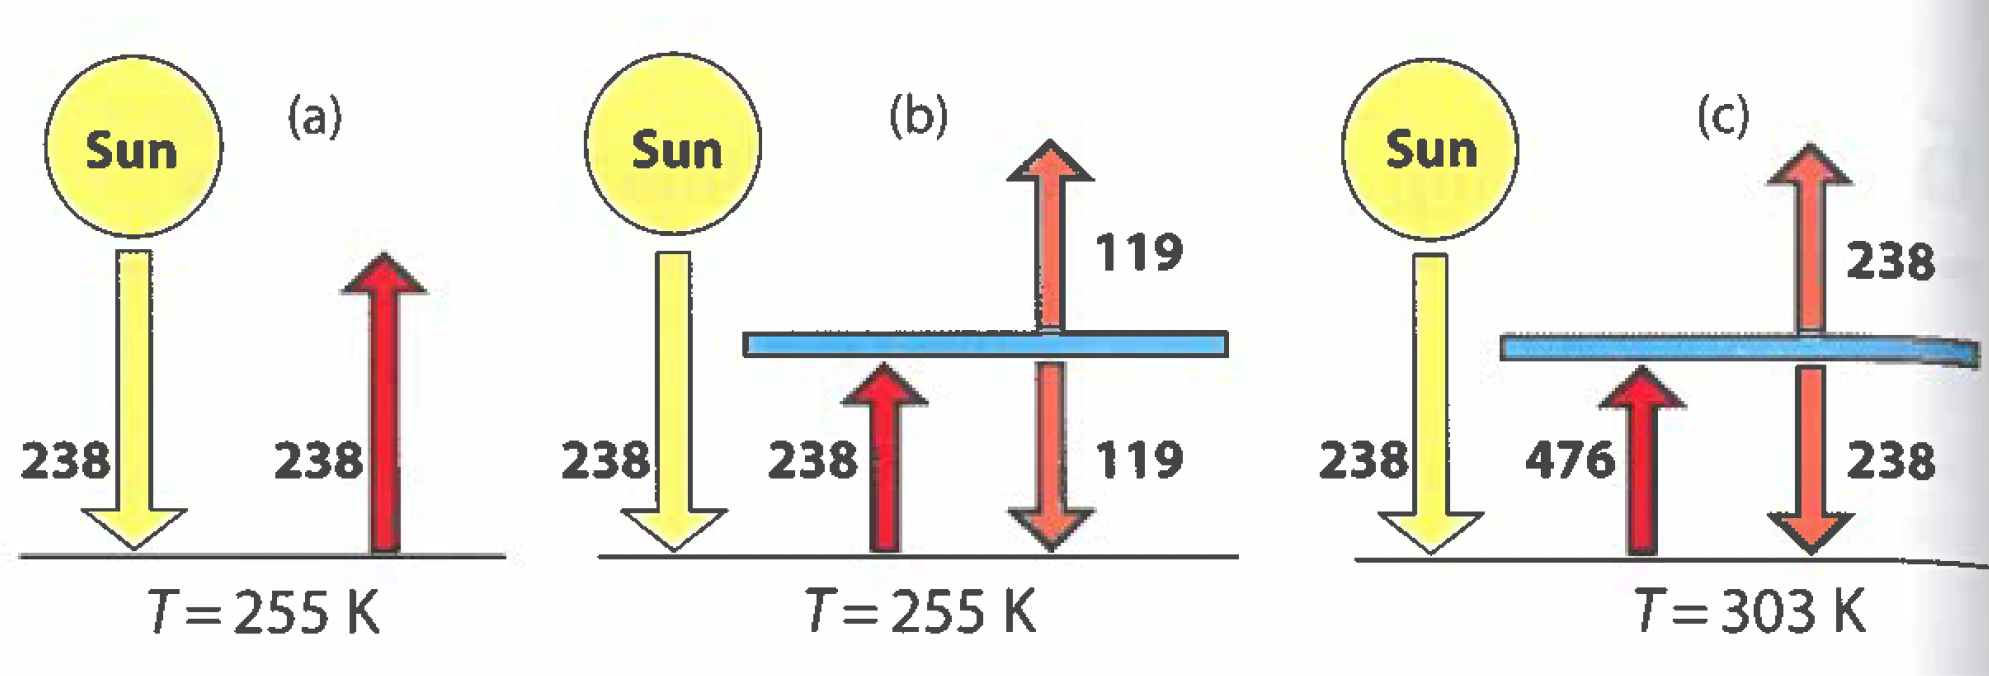
\includegraphics[width=\textwidth]{images/dessler_fig6-1_no-caption}

\caption{  \label{fig:dessler-fig6-1}
Figure 6.1 from {\em Dessler}: (a) An energy flux diagram for an Earth with no atmosphere (in equilibrium). (b) The immediate imposition of an atmosphere which is able to capture the Earth surface's IR radiation and re-radiate it. (c) A return to equilibrium.
}
\end{figure}


\begin{figure}
\centering
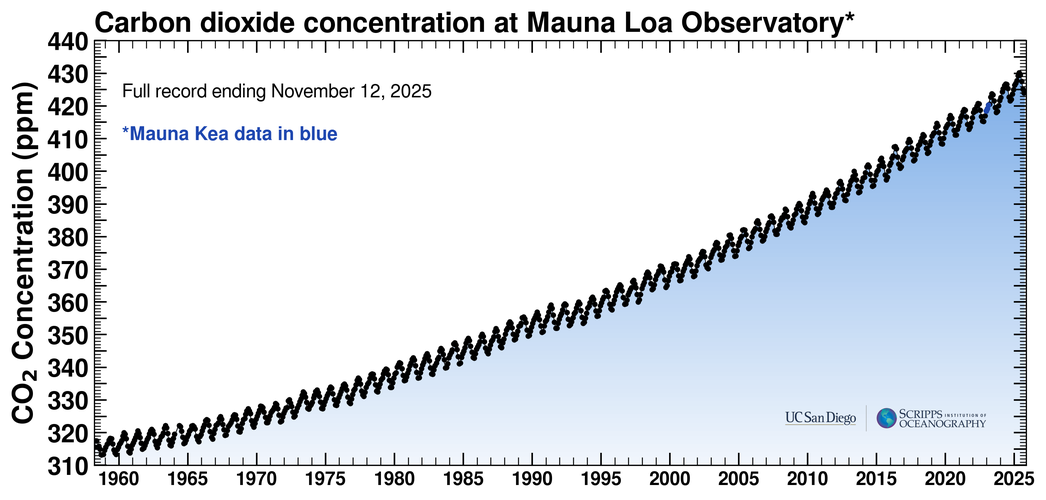
\includegraphics[width=\textwidth]{images/keeling-curve_mlo-full-record_2025-11-13.png}

\caption{ \label{fig:keeling-curve}
The so-called {\bf Keeling Curve} (named after Charles Keeling, who began atmospheric $\text{CO}_2$ measurements at Mauna Loa Observatory in Hawaii, in 1956) showing atmospheric carbon dioxide as a function of time.
}
\end{figure}


\begin{figure}
\centering
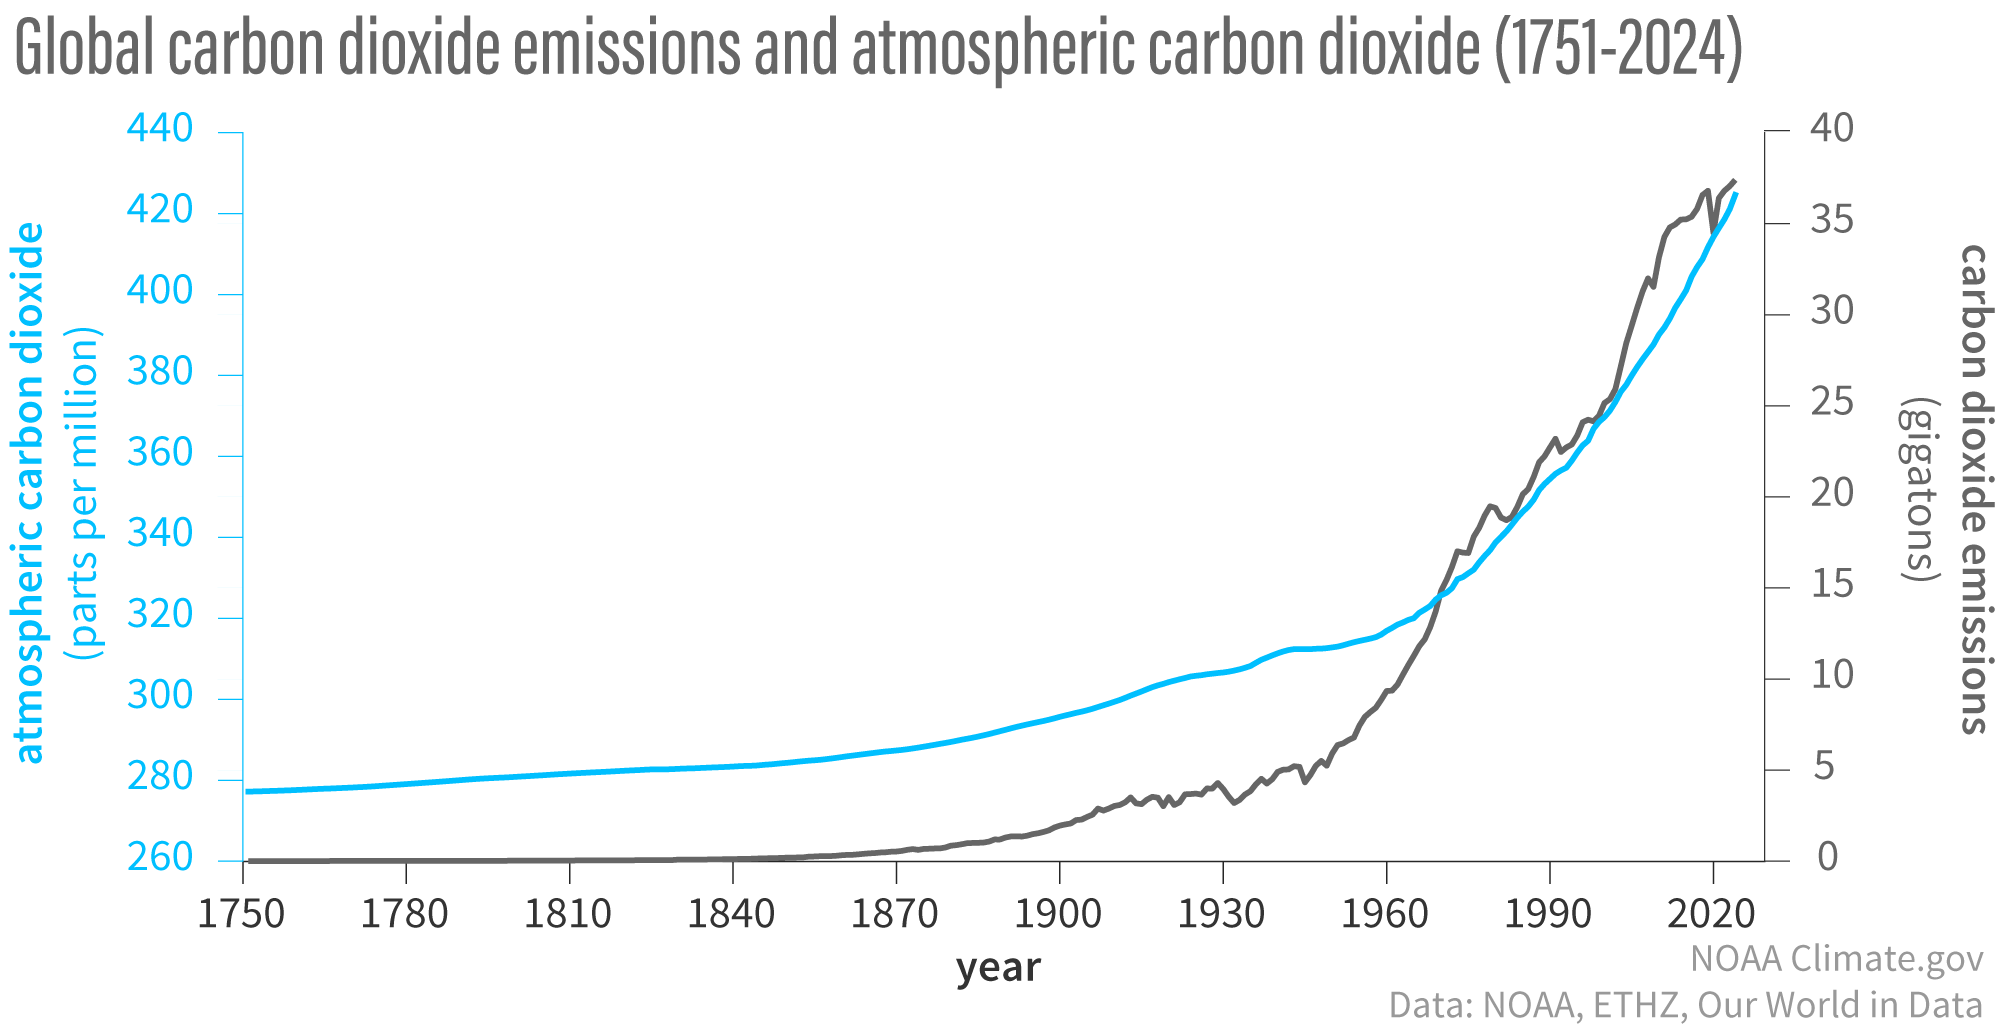
\includegraphics[width=\textwidth]{images/dashboard-carbon-dioxide-emissions-vs-atmospheric-concentration-1751-2024.png}

\caption{ \label{fig:co2-emissions-and-atmosphere}
Atmospheric carbon dioxide and emissions since the Industrial Revolution.
}
\end{figure}



\begin{figure}
\centering
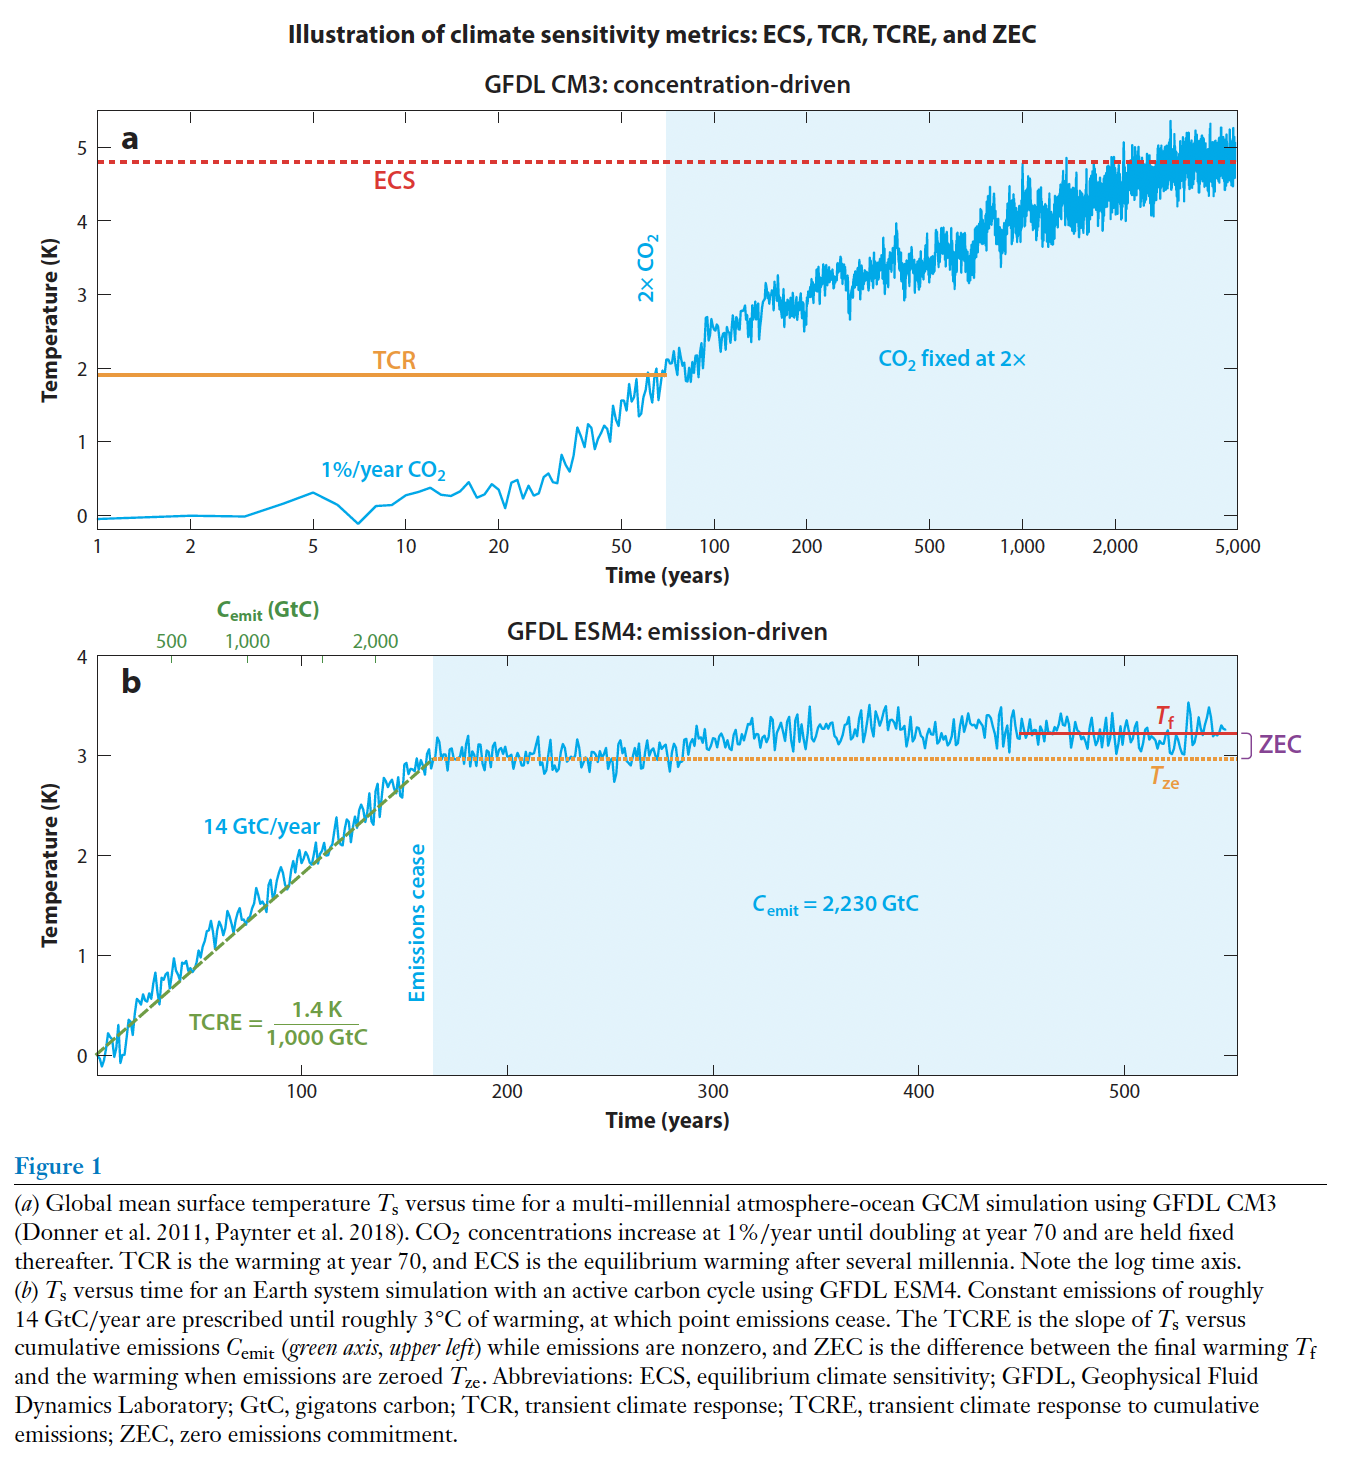
\includegraphics[width=\textwidth]{images/jeevanjee2025_fig1.png}

\caption{ \label{fig:jeevanjee-2025-review_fig1} 
Two pathways to the future.
}
\end{figure}





%%%%%%%%%%%%%%%%%%%%%%%%%%%%%%%%%%%%%%%%%%%%%%%%%%%%
%%%%%%%%%%                                  References                                %%%%%%%%%%%%%%%%
%%%%%%%%%%%%%%%%%%%%%%%%%%%%%%%%%%%%%%%%%%%%%%%%%%%%
%\noindent {\bf Data Sources}: 



\end{document}
